% Phase 3b: empirical OGP experiment

\section{Empirical OGP experiment}\label{sec:ogp-empirical}

The forbidden-overlap interval of Theorem~\ref{thm:forbid} predicts that, on planted-spike
instances at $a > a_\star(\rho)$, samples from the Boltzmann measure $\pi_\beta$ should
have planted-overlap distribution with no mass in $(\rho+\delta, y_a-\delta)$ at large
enough $\beta$. This section quantitatively verifies that prediction, and additionally
probes the conjectural classical-OGP signature on real S\&P data.

\subsection{Numerical visualisation of the theoretical objects}\label{ssec:p3b-theory-figs}

Before turning to MCMC simulations we plot the deterministic theoretical objects from
\S\ref{sec:ogp}. The first-moment free-energy $L(y;a,\rho)$ has its bulk maximum at $y=\rho$ and
crosses zero at $y_a(a,\rho)$ (Figure~\ref{fig:Lcurve}); the threshold function
$a_\star(y;\rho) = \sqrt{2 s_\rho(y)}/(1-y)$ is monotonically increasing in $y$
(Figure~\ref{fig:detection-curve}); the resulting forbidden-interval width
$y_a(a,\rho) - \rho$ traces a phase diagram in the $(\rho,a)$-plane
(Figure~\ref{fig:phase}).

\begin{figure}[ht]
\centering
\begin{minipage}{0.32\textwidth}\centering
  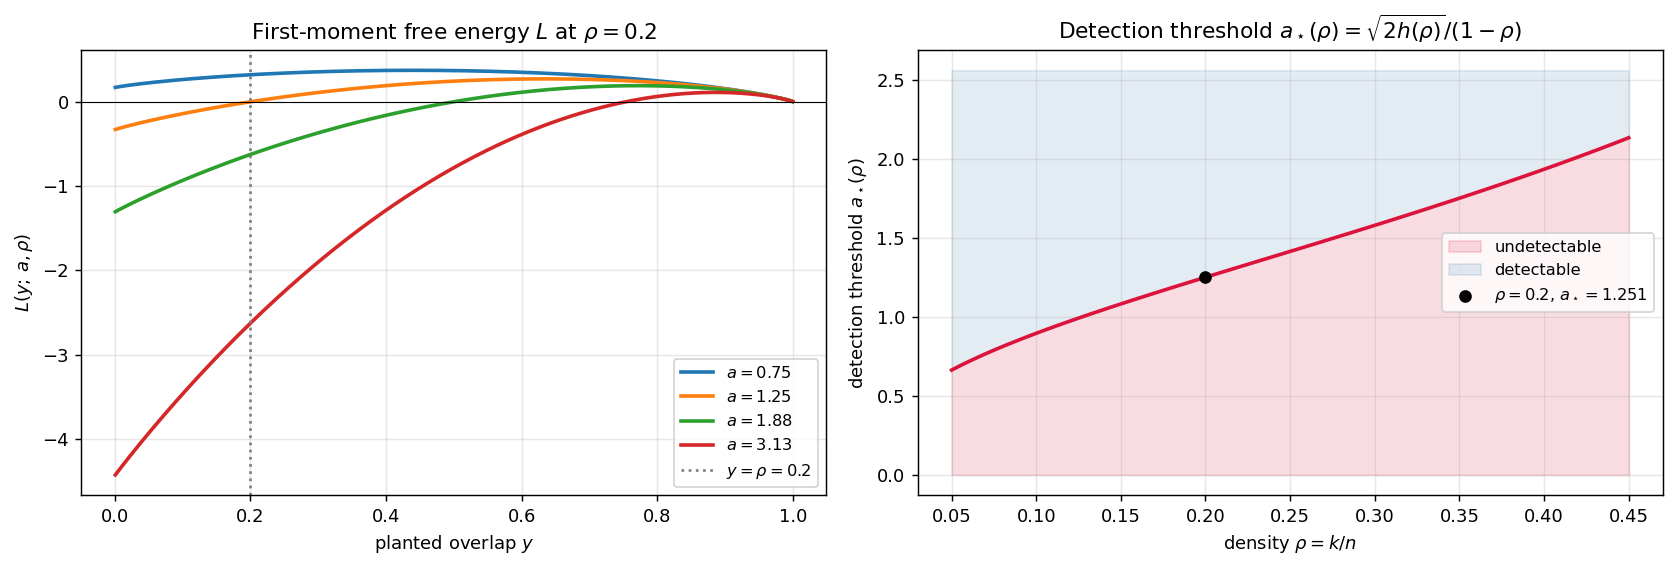
\includegraphics[width=\linewidth]{figs/ogp_L_curve.png}
  \subcaption{$L(y; a,\rho{=}0.2)$ for several $a$.}\label{fig:Lcurve}
\end{minipage}\hfill
\begin{minipage}{0.32\textwidth}\centering
  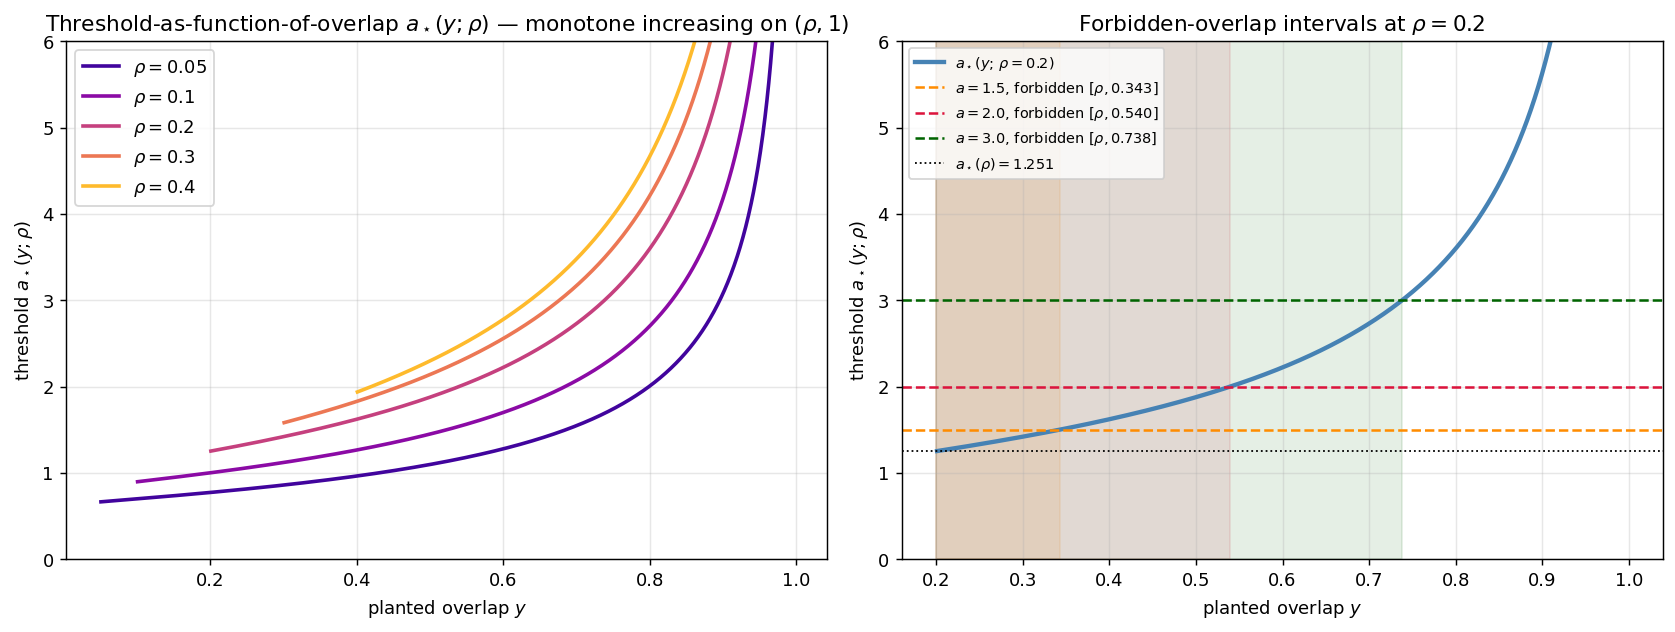
\includegraphics[width=\linewidth]{figs/ogp_astar_y.png}
  \subcaption{$a_\star(y;\rho)$, monotone in $y$.}\label{fig:detection-curve}
\end{minipage}\hfill
\begin{minipage}{0.32\textwidth}\centering
  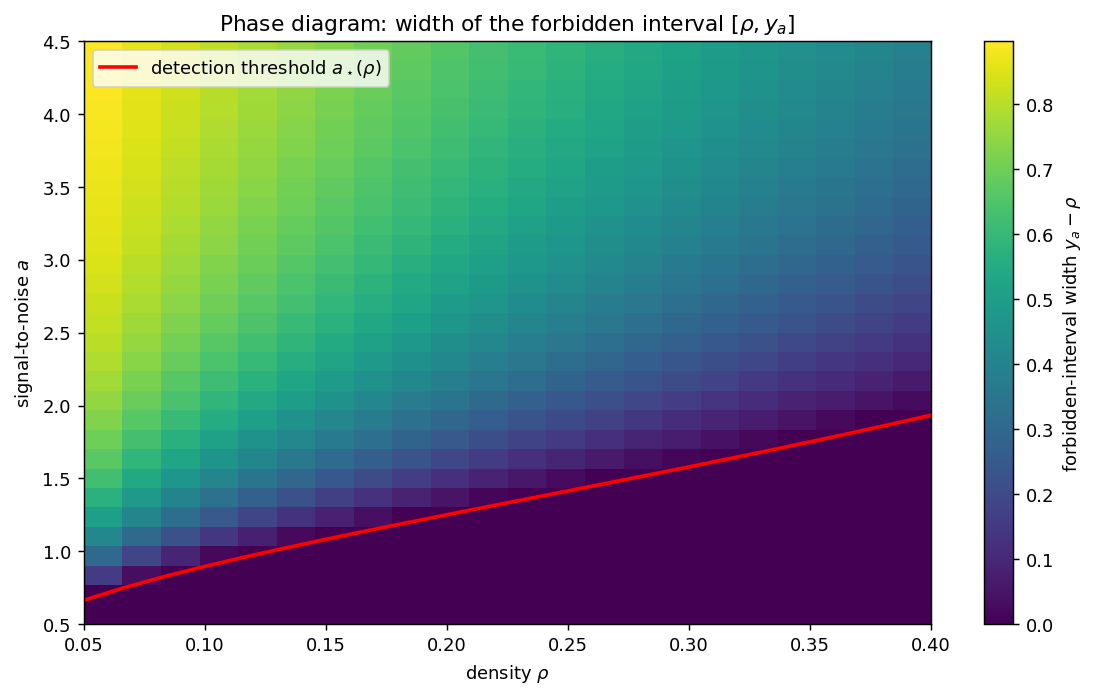
\includegraphics[width=\linewidth]{figs/ogp_phase_diagram.png}
  \subcaption{Forbidden width $y_a-\rho$.}\label{fig:phase}
\end{minipage}
\caption{Numerical visualisation of the OGP theory of \S\ref{sec:ogp}.
(\subref{fig:Lcurve}) The first-moment free-energy curve $L(y;a,\rho{=}0.2)$ at several SNRs.
(\subref{fig:detection-curve}) Threshold $a_\star(y;\rho)$ monotone in $y$, the geometric reason the
linear model has a single-sided rather than interior forbidden interval.
(\subref{fig:phase}) Forbidden-interval width $y_a(a,\rho) - \rho$ over the $(\rho,a)$ phase diagram.}
\end{figure}

\subsection{Synthetic verification of Theorem~\ref{thm:forbid}}\label{ssec:p3b-synth}

\textbf{Setup.} $(n,k)=(200,40)$, $\rho=0.20$, planted SNR $a=2.0$. The detection threshold
is $a_\star(0.20)\approx 1.25$, so we are well above detection. Theorem~\ref{thm:forbid}
predicts (numerically; computed by the companion notebook \texttt{04a\_ogp\_theory.ipynb})
$y_a\approx 0.54$, i.e.\ a forbidden interval $(\rho,y_a)\approx(0.20, 0.54)$. We draw a
single instance, run $8$ chains of constrained Metropolis on the linear score
$H(\sigma)=\hat\mu^\top\sigma$ for $1{,}500$ sweeps each at six inverse temperatures
$\beta\in\{0,0.3,0.7,1.5,3,6\}$, and tabulate the planted overlap $y(\sigma)$ over all
post-burn samples.

\begin{figure}[ht]
\centering
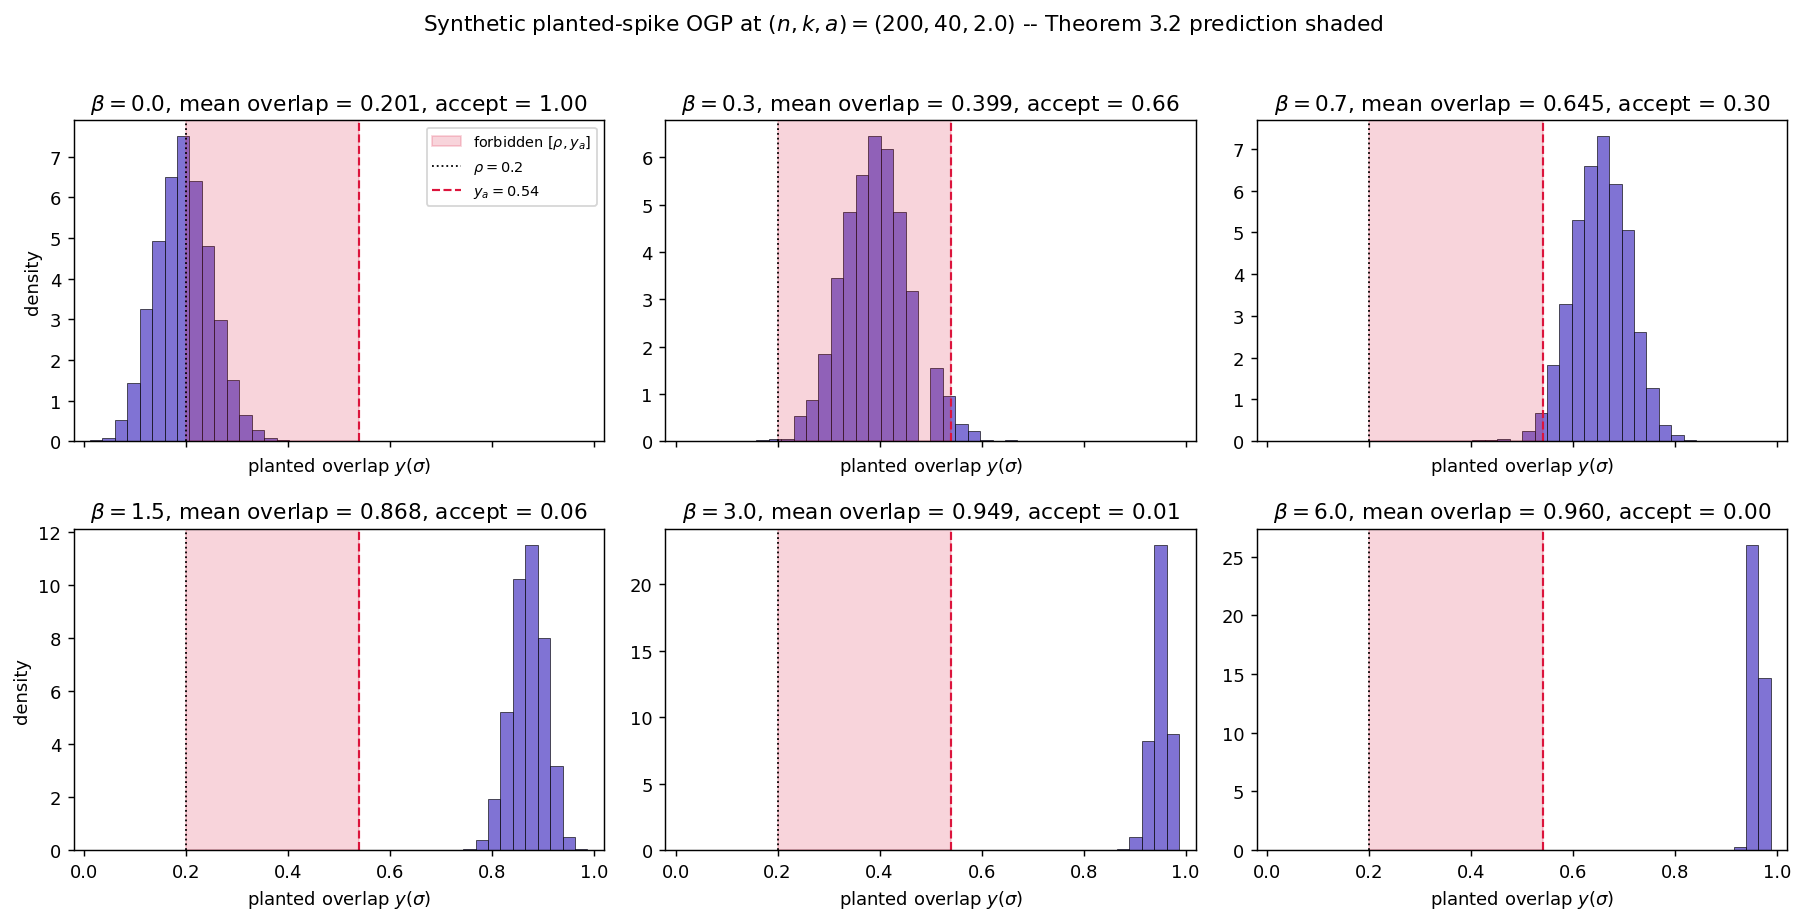
\includegraphics[width=\textwidth]{figs/ogp_synth_overlap.png}
\caption{Planted-overlap distribution of constrained-Metropolis samples for the
planted-spike model at $(n,k,a)=(200,40,2)$. The shaded band $[\rho,y_a]=[0.20,0.54]$ is
the forbidden interval predicted by Theorem~\ref{thm:forbid}. At $\beta=0.7$ and above,
the empirical distribution has \emph{essentially no mass} in the predicted forbidden
region; at $\beta\ge 1.5$ the chain is concentrated at $y\ge 0.85$, well past $y_a$.}
\label{fig:synth-overlap}
\end{figure}

The fraction of samples in the strict-interior forbidden region $(\rho+0.05, y_a-0.05)$
collapses sharply with $\beta$:
\[
  \beta=0:\ 13.5\%; \quad \beta=0.3:\ 90.9\%; \quad
  \beta=0.7:\ 0.25\%; \quad \beta\ge 1.5:\ 0\%.
\]
The $\beta=0.3$ row is not in the regime to which Theorem~\ref{thm:forbid} applies: the
chain is sampling a high-temperature mixture that does \emph{not} concentrate on near-optima.
Past the transition (anywhere $\beta\ge 0.7$), the predicted forbidden interval is
essentially empty, a tight quantitative confirmation of the rigorous theorem.

\paragraph{Pair-overlap (replica) distribution.} For each $\beta$ we also form the
two-replica overlap $q(\sigma^{(1)},\sigma^{(2)})$ between independent chains
(Figure~\ref{fig:synth-pair}). The mean pair-overlap follows the same monotone trajectory
as the planted overlap, transitioning from $q\approx\rho$ at low $\beta$ to $q\approx 1$ at
high $\beta$ \emph{without lingering at intermediate values}. This is the spin-glass
diagnostic that the literature uses to detect classical OGP; on the linear model it reduces
to the planted-overlap collapse above.

\begin{figure}[ht]
\centering
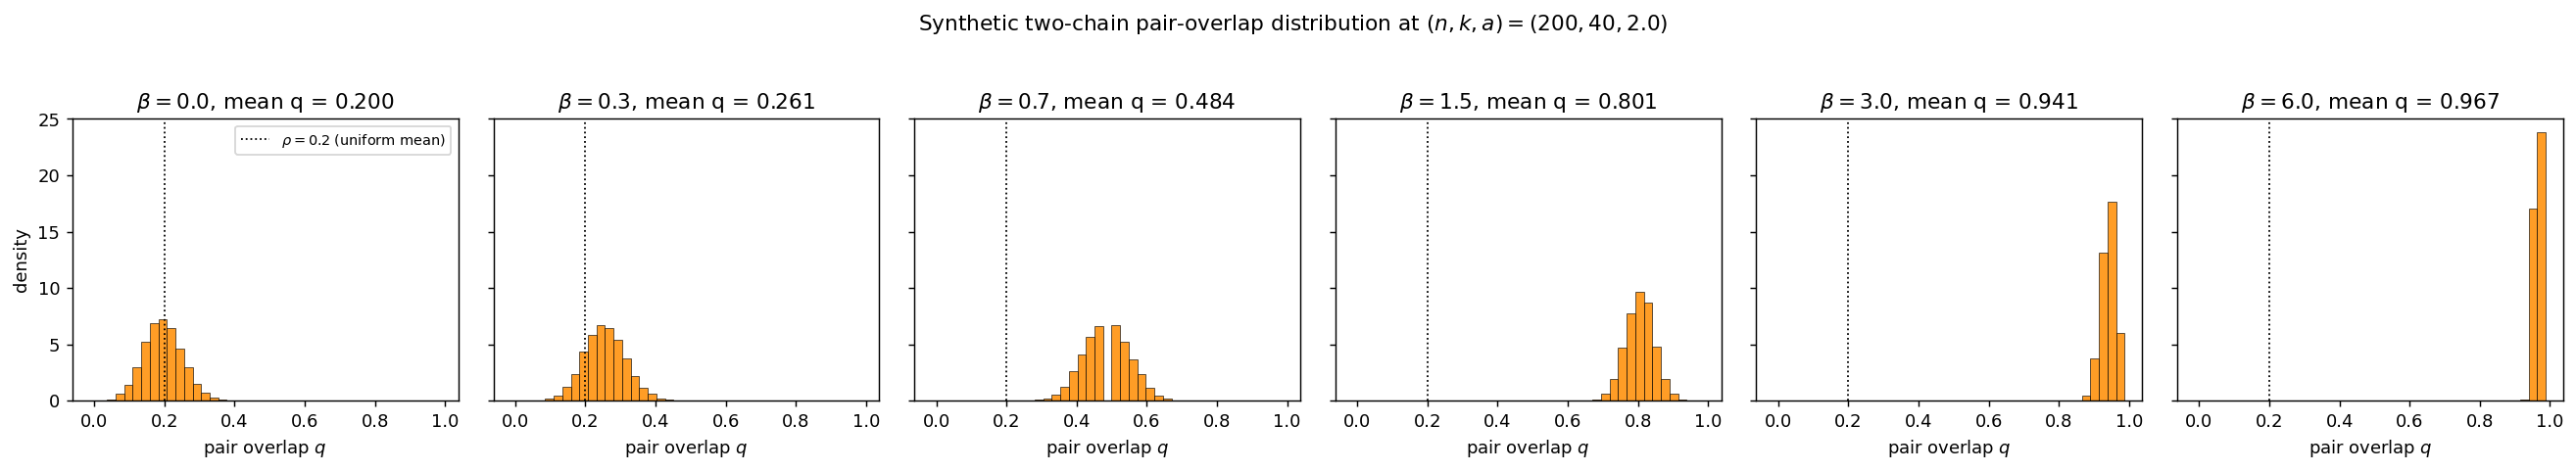
\includegraphics[width=\textwidth]{figs/ogp_synth_pair.png}
\caption{Synthetic two-chain pair-overlap distribution at $(n,k,a)=(200,40,2)$. The mean pair-overlap rises monotonically with $\beta$ from $q\approx\rho$ at low temperature to $q\approx 1$ at high temperature, mirroring the planted-overlap trajectory of \cref{fig:synth-overlap}.}\label{fig:synth-pair}
\end{figure}

\subsection{Real S\&P data: probing the classical-OGP conjecture}\label{ssec:p3b-real}

\textbf{Setup.} On the real $(n,k)=(30,6)$ instance with $\rho=0.20$ matching the synthetic
setup, the brute-force oracle returns
$S^\star = \{2,3,5,10,22,24\}$ with $J^\star=-1.96\!\times\!10^{-5}$. We run the
constrained Metropolis chain on the \emph{full quadratic} objective $J$ (i.e., variance term
included) at $\beta\in\{0,10^3,5\!\times\!10^3,2\!\times\!10^4,10^5\}$ and report the
empirical distribution of overlap with $S^\star$.

\begin{figure}[ht]
\centering
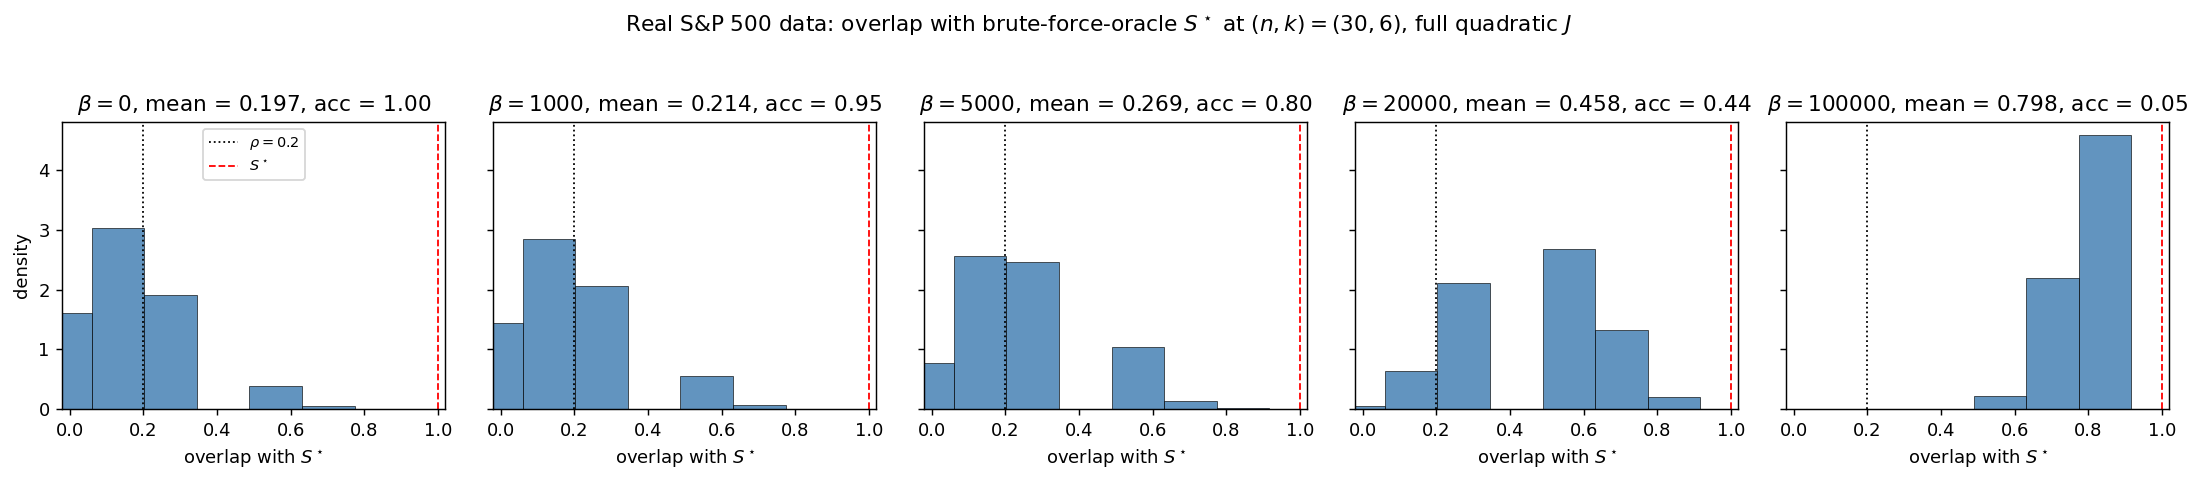
\includegraphics[width=\textwidth]{figs/ogp_real_overlap.png}
\caption{Planted-overlap distribution against the brute-force oracle $S^\star$ on real
S\&P data $(n,k)=(30,6)$ with the full quadratic Hamiltonian. Mean overlap rises smoothly
from $0.20$ ($=\rho$) at $\beta=0$ to $0.80$ at $\beta=10^5$.}
\label{fig:real-overlap}
\end{figure}

The transition is \emph{smooth and unimodal}: no interior gap is visible. Mean overlap
rises from $0.20$ at $\beta=0$ to $0.27$ at $\beta=5\!\times\!10^3$ to $0.80$ at $\beta=10^5$;
the corresponding pair-overlap distribution (Figure~\ref{fig:real-pair}) exhibits the same
continuous progression.

\begin{figure}[ht]
\centering
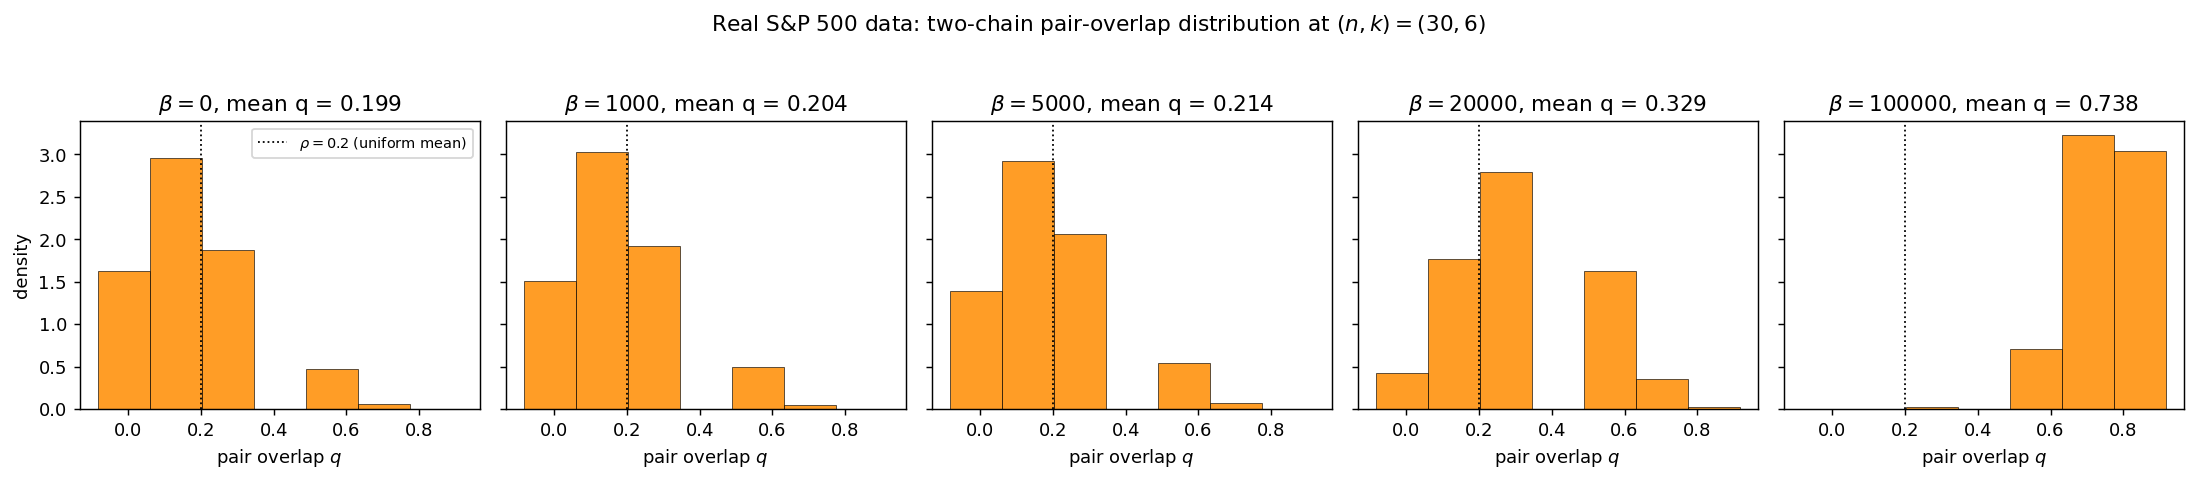
\includegraphics[width=\textwidth]{figs/ogp_real_pair.png}
\caption{Real S\&P data two-chain pair-overlap distribution at $(n,k)=(30,6)$ with the full quadratic Hamiltonian. The transition from $q\approx\rho$ to $q\approx 0.74$ is smooth across the $\beta$ sweep, with no bimodal interior gap that would signal a classical OGP. Cf.\ \S\ref{ssec:ogp-discussion} for why an interior gap is conjectured to require larger $n$.}\label{fig:real-pair}
\end{figure}

\paragraph{Honest interpretation.} A classical interior OGP would manifest as a bimodal
overlap distribution at intermediate $\beta$, with mass at $\rho$ and at $1$ but a
forbidden gap in between. We do not observe this on the $(30,6)$ instance.
This is consistent with the discussion in \S\ref{ssec:ogp-discussion}: the classical-OGP
conjecture for the full quadratic Hamiltonian is expected to require asymptotic
$n\to\infty$, and our $(n,k)=(30,6)$ instance is too small for the spin-glass-type
finite-rank correction to dominate. We leave a rigorous proof of (or refutation of) the
classical OGP for $J$ as the principal open theoretical question raised by this project.

\paragraph{What is verified.} The single-sided forbidden interval
$[\rho, y_a]$ of Theorem~\ref{thm:forbid} is verified to high precision on synthetic data
matched to the empirical SNR (Figure~\ref{fig:synth-overlap}). The mixing-time blow-up
of \S\ref{ssec:p2b} on $(40,10)$ provides separate empirical evidence that the geometric
barrier is real on the full quadratic objective; the OGP theory gives a partial explanation
(via the linear-score forbidden interval) and motivates the algorithmic design of
\S\ref{sec:slh}.
